\chapter{Web Testing with Selenium 1}
Selenium, with its official name "The Selenium Browser Automation Project", is an umbrella project for various tools and libraries that automates certain web browser tasks according to the definition in the official website\footnote{\url{https://www.selenium.dev/documentation/}}. Selenium is a gateway to access browser features from a programming language through various language bindings. It presents a consistent API to access those features. An example that opens the official Selenium website is given in Listing \ref{lst:selenium-example} with Java programming language.

\begin{lstlisting}[language=java,caption={A Java program that opens the official Selenium website through a Chrome-based browser.}, label=lst:selenium-example]
import org.openqa.selenium.WebDriver;
import org.openqa.selenium.chrome.ChromeDriver;

public class HelloSelenium {
    public static void main(String[] args) {
        WebDriver driver = new ChromeDriver();

        driver.get("https://selenium.dev");

        driver.quit();
    }
}
\end{lstlisting}

At its core Selenium has a WebDriver. Once it has been installed, all Chromium and Gecko-based browsers can be controlled with a few lines of code through six different programming languages. One of these programming languages is, not surprisingly, Java. In this section, installation steps and a few examples to introduce the basics of Selenium are covered.

\section{Installation}
There are two ways to work with Selenium. With the first one, you have to install the language binding libraries for your language of choice, the browser you want to use, and the driver for that browser. This is the seemingly more professional way to work with Selenium. The other way to work is to install the Selenium IDE\footnote{\url{https://www.selenium.dev/selenium-ide/}}. Selenium IDE provides a record-and-replay style workflow. It is easier to work with and it is not required to write code.

It is straightforward to install the Selenium library for Java with Maven. Just add the Selenium dependency which is shown in the code snippet in Listing \ref{lst:selenium-dep} to the \lstinline[language={}]!pom.xml! file.

\begin{lstlisting}[language=XML,caption={The Selenium dependency for Maven.},label=lst:selenium-dep]
<dependency>
  <groupId>org.seleniumhq.selenium</groupId>
  <artifactId>selenium-java</artifactId>
  <version>4.0.0</version>
</dependency>
\end{lstlisting}

After that, the WebDriver of choice should be installed. Notice that the major version number of the WebDriver must match with the major version number of the installed browser. All WebDriver utilities are provided by the vendor themselves and should be downloaded from their official websites\footnote{\url{https://www.selenium.dev/documentation/webdriver/getting\_started/install\_drivers/}}. The installed WebDriver should be visible on PATH. Each operating system has a different way to maintain PATH. In Linux, if the WebDriver is installed via a package manager, no further action is needed since most package managers automatically create symbolic links to the directories which are scanned by default. Alternatively, it is possible to use the installed driver by hard-coding the driver path. Example of it is given in the code snippet in Listing \ref{lst:selenium-hc-path}.

\begin{lstlisting}[language=java,caption={Using the driver from a hard-coded path.},label=lst:selenium-hc-path]
System.setProperty("webdriver.chrome.driver","/path/to/chromedriver");
ChromeDriver driver = new ChromeDriver();
\end{lstlisting}

\subsection{Detailed Steps for Selenium Installation}

\begin{figure}
    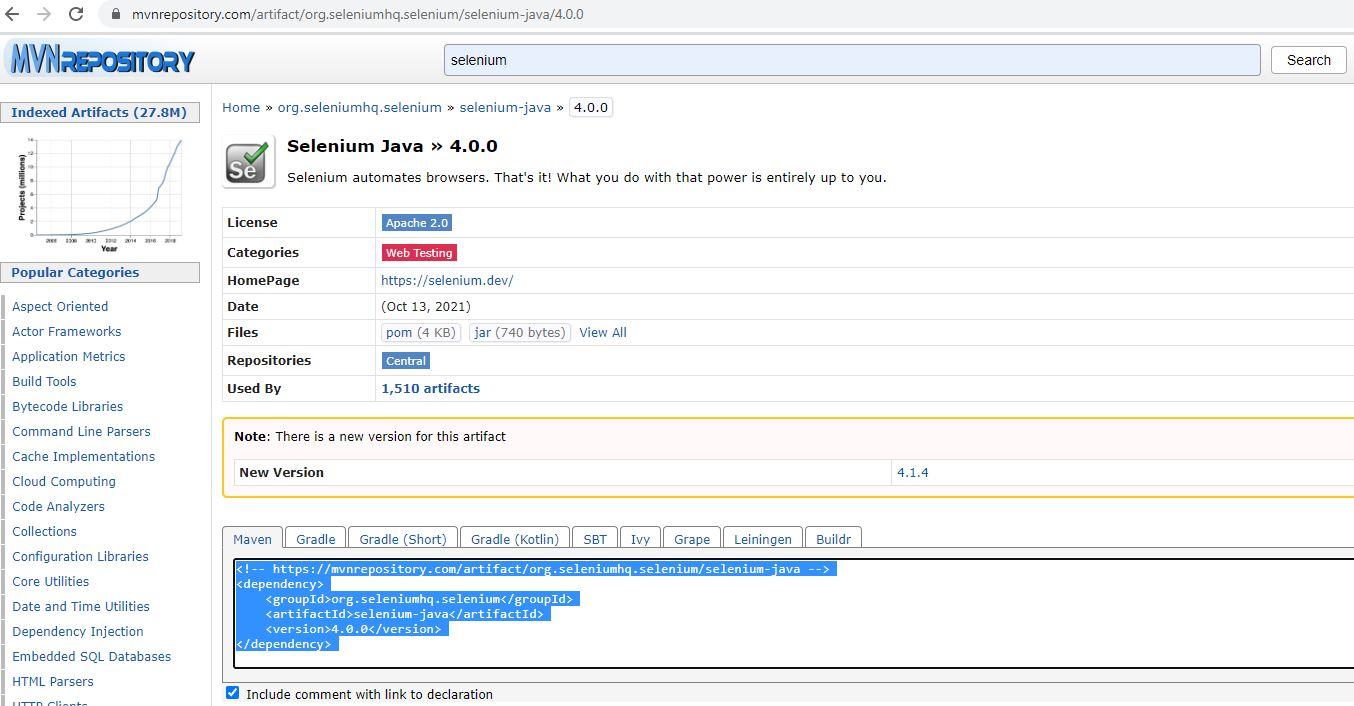
\includegraphics{images/selenium1-detailed-install-1.jpg}
    \caption{Selenium dependency on the Maven repository website.}
    \labfig{sel-dep-maven-webite}
\end{figure}

\begin{enumerate}
    \item Create a Maven project as described in Chapter 10. Make sure to update the pom.xml file and change the Java compiler version.
    \item Add the Selenium dependency also to the pom.xml file of the project (between 'dependencies' tags). To find the dependency:
    \begin{enumerate}
        \item Go to the website of Maven Repository.
        \item Search for "Selenium" and select "Selenium Java" option.
        \item Select the version 4.0.0 and copy the dependency on the opened page, which is displayed in \reffig{sel-dep-maven-webite}.
    \end{enumerate}
    \item Install a WebDriver according to the browser you use (e.g. Chrome). For downloading the WebDriver:
    \begin{enumerate}
        \item Go the the website of Selenium, using the link \url{https://bit.ly/39iaKXU}.
        \item On the opened page that is shown in \reffig{sel-install-page-webite}, according to the browser you use, click the “Downloads” section.
    \end{enumerate}
    \item Select the proper option on the opened page, considering the key points described below:
    \begin{enumerate}
        \item Find the current version of the browser you use. The leftmost number of the version is its major version.
        \item Find the WebDriver option that has the same major version as your browser, and download it.
        \item It will be downloaded as a .zip file, so finally extract the webdriver.
    \end{enumerate}
    \item Now, you are ready to work with Selenium and try the exercises on the lab manual.
\end{enumerate}

\begin{figure}
    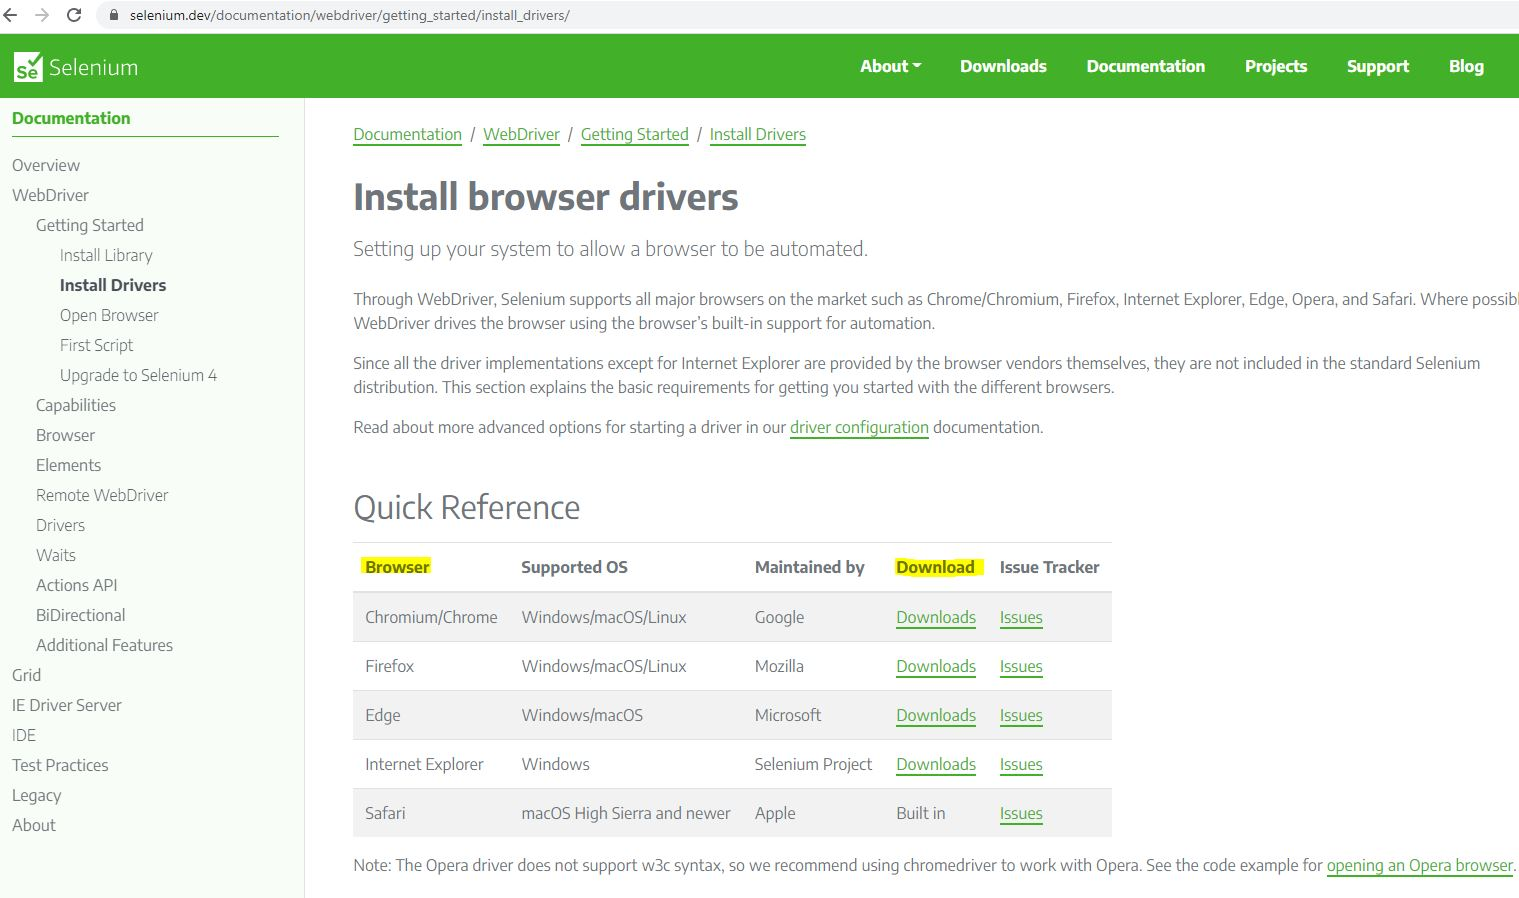
\includegraphics{images/selenium1-detailed-install-2.jpg}
    \caption{WebDriver installation page of the Selenium website.}
    \labfig{sel-install-page-webite}
\end{figure}

\section{Usage}
In this section, it is assumed that Google Chrome is the choice of browser. Therefore, Chrome WebDriver should be installed. After installing the Selenium library, the browser, and the relevant WebDriver, you can open the Selenium-controlled browser with the following code snippet.

\begin{lstlisting}[language=java,caption={Start a Selenium-controlled browser instance.}]
ChromeOptions options = new ChromeOptions();
driver = new ChromeDriver(options);

driver.quit();
\end{lstlisting}

By default, Selenium 4 is compatible with Chrome v75 and greater. Note that the version of the Chrome browser and the version of chromedriver must match the major version. In addition to the shared capabilities, there are specific Chrome capabilities that can be used. Let's break down and extend the code.

The following code snippet opens a Selenium-controlled browser instance with default options.
\begin{lstlisting}[language=java]
WebDriver driver = new ChromeDriver();
\end{lstlisting}

This code snippet opens the given web page on the browser.
\begin{lstlisting}[language=java]
driver.get("https://selenium.dev");
\end{lstlisting}

One can access all of the attributes about an opened web page through the driver variable. In the following code snippet, the title of the web page is accessed.
\begin{lstlisting}[language=java]
driver.getTitle(); // => "Google"
\end{lstlisting}

Synchronizing the code with the current state of the browser is one of the biggest challenges with Selenium, and doing it well is an advanced topic. Essentially you want to make sure that the element is on the page before you attempt to locate it and the element is in an interactable state before you attempt to interact with it. An implicit wait is rarely the best solution, but it’s the easiest to demonstrate here, so we’ll use it as a placeholder.
\begin{lstlisting}[language=java]
driver.manage().timeouts().implicitlyWait(Duration.ofMillis(500));
\end{lstlisting}

The majority of commands in most Selenium sessions are element related, and you can’t interact with one without first finding an element.
\begin{lstlisting}[language=java]
WebElement searchBox = driver.findElement(By.name("q"));
WebElement searchButton = driver.findElement(By.name("btnK"));
\end{lstlisting}

There are only a handful of actions to take on an element, but you will use them frequently.
\begin{lstlisting}[language=java]
searchBox.sendKeys("Selenium");
searchButton.click();
\end{lstlisting}

Elements store a lot of information that can be requested. Notice that we need to relocate the search box because the DOM has changed since we first located it.
\begin{lstlisting}[language=java]
driver.findElement(By.name("q")).getAttribute("value"); // => "Selenium"
\end{lstlisting}

This ends the driver process, which by default closes the browser as well. No more commands can be sent to this driver instance.
\begin{lstlisting}[language=java]
driver.quit();
\end{lstlisting}

Let’s combine these previous things into a complete script.
\begin{lstlisting}[language=java,caption={The complete example to open Google and search for Selenium.}]
import org.openqa.selenium.By;
import org.openqa.selenium.WebDriver;
import org.openqa.selenium.WebElement;
import org.openqa.selenium.chrome.ChromeDriver;

public class HelloSelenium {
    public static void main(String[] args) {
        driver = new ChromeDriver();

        driver.get("https://google.com");
        
        driver.getTitle(); // => "Google"

        driver.manage().timeouts().implicitlyWait(Duration.ofMillis(500));
        
        WebElement searchBox = driver.findElement(By.name("q"));
        WebElement searchButton = driver.findElement(By.name("btnK"));
        
        searchBox.sendKeys("Selenium");
        searchButton.click();
        
        searchBox = driver.findElement(By.name("q"));
        searchBox.getAttribute("value"); // => "Selenium"
        
        driver.quit();
    }
\end{lstlisting}

WebDriver drives a browser natively, as a user would, either locally or on a remote machine using the Selenium server, marks a leap forward in terms of browser automation. More information on the API can be found in the documentation\footnote{\url{https://www.selenium.dev/documentation/webdriver/}}.

Several configuration changes need to be made to run the program from the \lstinline!main(String[])! function. The first one is to add the fully qualified class name of the class that contains the main function. It is marked as \lstinline!mainClass! variable in the \lstinline!pom.xml! file. Add the following code snippet inside of the \lstinline[language=XML]!<properties>! element after the compiler target element:
\begin{lstlisting}[language=XML]
<exec.mainClass>the.package.name.HelloSelenium</exec.mainClass>
\end{lstlisting}

Here, the package name can be nothing or the package name that is indicated at the first line of the main class. Now, we need to tell Eclipse to build and run the program without running the tests when we send the command Maven build. If tests are run after a successful build, make sure that they all pass. Otherwise, the build will fail.

To create a build and run without tests config, right-click to the project. From the context menu, choose \menu{Run As > Run Configurations...}. A dialog box should appear. In the dialog, right-click to the Maven Build and choose \menu{New Configuration}. This should create a configuration similar to Figure \ref{fig:run-configs}. In the Goals textbox, write \lstinline[language={}]!clean install exec:java!. Finally, tick the \lstinline[language={}]!Skip Tests! checkbox. Click \emph{Apply}, then \emph{Run} buttons. If everything works correctly, a browser window should appear and search for "Selenium" in Google, and close.

\begin{figure}[H]
    \centering
    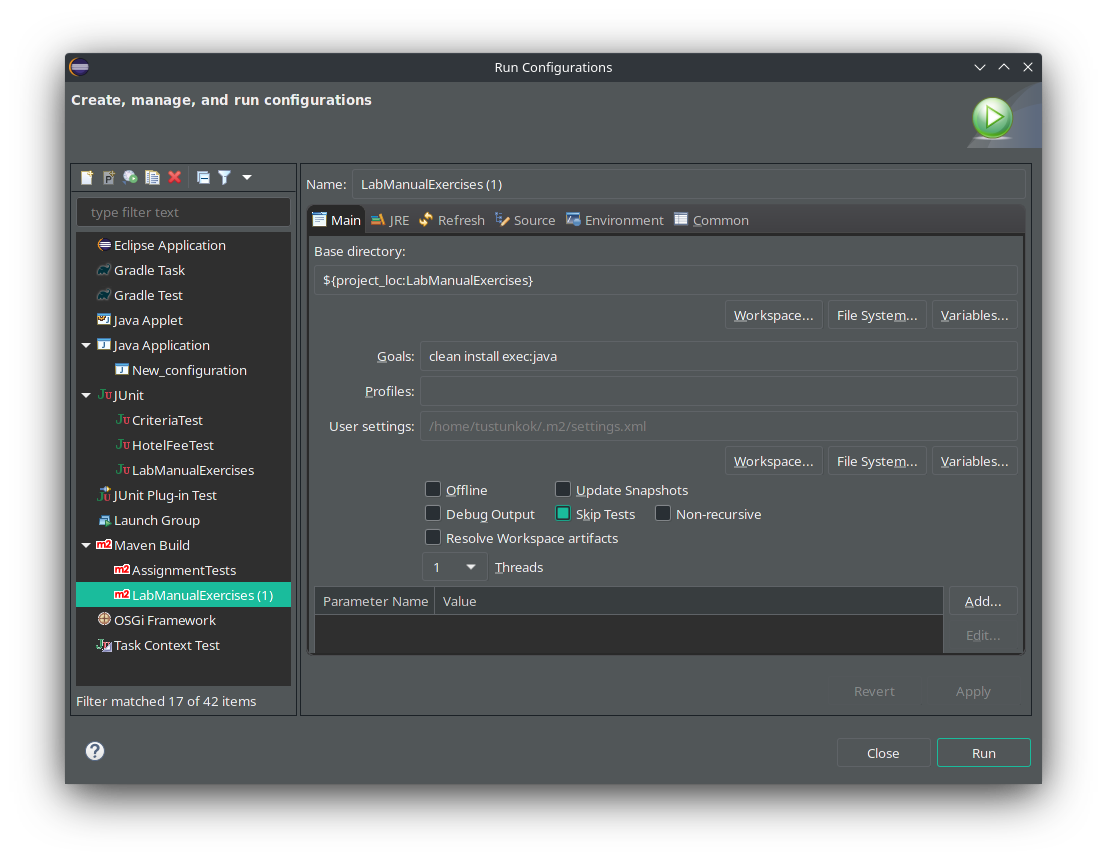
\includegraphics[width=\textwidth]{images/maven-run-config.png}
    \caption{Run configurations dialog window.}
    \label{fig:run-configs}
\end{figure}